\documentclass[11pt,twoside,a4paper]{article}

\usepackage{a4wide,amsmath,amssymb}

% Mann will direkt Umlaute eingeben können statt \"a, \"o, \"u usw.
% Entweder:
\usepackage[utf8]{inputenc}
% oder:
%\usepackage{umlaut}
\usepackage[german]{babel}

\usepackage{textcomp}
\usepackage{graphicx}
\usepackage{subcaption}

\usepackage{hyperref}


% Trennvorschl"age (in {} einfuegen, wenn nicht automatisch getrennt wird:
% z.B. Authen-ti-ka-tions-sys-tem)
%\hyphenation{}

%\hyphenation{min-des-tens}
%\hyphenation{Kol-li-sions-er-ken-nung}


%-------------------------- Formatsachen --------------------------%

% Bild-, Tabellenunterschriften veraendern:
% Nummer fett, kleinerer Text fuer Bildunterschrift
%\usepackage[bf,small]{caption}


%\usepackage{mathpazo}  % -- Palatino als Zeichensatz -- einfach diese
					   % Zeile auskommentieren, falls nicht installiert
%\usepackage{mathptmx}  % -- Times als Zeichensatz

% Zum Unterscheiden von Entwurfs- und endgueltiger Fassung
%\usepackage{draftcopy}
%\draftcopySetGrey{0.90}   %   90% = sehr helles Grau
%\draftcopyName{ENTWURF}{155}   % statt ``DRAFT''
%\draftcopySetScale{1}

%--------------- Zeilen- und Absatzabstaende ----------------------%
%\setlength{\parindent}{0em}
%\setlength{\parskip}{\medskipamount}    % Abstand zwischen Abs"atzen

\begin{document}

\title{HSP-Projektarbeit im Master Informatik \\
\small Kollisionsdetektion in in Echtzeit gerenderten 3D-Simulationen mit Fokus auf die Verwendung in Videospielen}
\author{Robert Graf, Lukas Hermann\\
%  (\texttt{fridolw@in.tum.de})\\[5mm]
%  Seminar "`Internetrouting"' , \\
  Ostbayerische Technische Hochschule Regensburg\\
  \\
  Projektbetreuung: Prof. Dr. Klaus Volbert
}
  
\date{WS\, 2019/2020 (Version vom \today)}


\maketitle

\newpage
\tableofcontents


\abstract{Dieses Projekt umfasst die Erstellung einer 3D-Simulation mit dem Fokus auf die Implementierung von Algorithmen zur Kollisionserkennung von rigiden 3D-Objekten. In diesem Bericht werden verschiedene Ansätze behandelt als auch Probleme und Hürden in der Bearbeitung dargestellt.}


\section{Einleitung}

Dieses Dokument dient als Spezifikation für ein 3D-Simulationsprogramm, welches für die Umsetzung diverser Videospielideen konzipiert ist.
Es sollen ausgewählte Aspekte der Simulation deklarativ beschrieben und/oder spezifiziert werden, ohne eine spezifische Umsetzung zu sehr einzuschränken.
Das Dokument kann ebenfalls detaillierte Informationen zur derzeitigen Umsetzung bestimmter Aspekte der Simulation liefern.
Weiter dient es als Leitfaden, in dem relevantes Kontextwissen gesammelt und referenziert ist.

\section{Problemdefinition}
Die 3D-Simulation umfasst hier die Echtzeitsimulation von Entitäten in einem 3D-Kontext. Darin enthalten sind ebenfalls die Aufgaben der Video- und Audioanzeige des Inhalts der Simulation und die Steuerung von bestimmten Inhalten in Echtzeit.\\
Die konkreten Ausmaße des Problems der Erstellung dieser Simulation ist von den Features der zu simulierenden Entitäten abhängig.

Um einen grundlegenden Einblick zu bieten können einige der umgesetzten, bzw. angestrebten Features für diese Simulation beispielhaft beschrieben werden.\\
Klassischerweise im Kontext der 3D-Simulation per se umfasst dies:
\begin{enumerate}
\item Rigide physikalische Objekte
\item passiv physikalische rigide Objektkollision
\end{enumerate}

Im Kontext eines Videospiels können weitere Aspekte hinzugefügt werden. Einige sind dabei abhängig vom jeweiligen zu realisierenden Videospiel:
\begin{enumerate}
\item Projektile
\item Nicht Spieler Charactere (NPC)/Gegner
\item Spieleravatare\\
Von einem Benutzer Steuerbare Entitäten, welche diverse Aktionen ausführen können.
\item Terrain
\item diverse benutzbare Gegenstände/Items und Inventare (Werkzeuge/Waffen)
\end{enumerate}


\section{Kontext \& Terminologie}
Das L0-Level (siehe \ref{l0}) beschäftigt sich mit der Datenrepräsentation von Modellen, Zeit und Raum.\\

Die Repr"asentation stellt sich dabei jedoch Anforderungen verschiedener technologischer Perspektiven:
		\begin{itemize}
			\item graphische Darstellung/Rendering
				F"ur die graphische Darstellung m"ussen bestimmte Formate eingehalten werden. Datenkonfomit"at mit graphischen Bibliotheken erspart umst"andliche Umwandlungen von Repr"asentationen.
			\item physikalische Berechnung
				F"ur die Kollisionsberechnung k"onnen bestimmte Repr"asentationen vorteilhaft sein. Die Repr"asentation versucht m"oglichst statisch Information "uber Objekte bereitzustellen und vermeidet dynamische Nachberechnung von Objekteigenschaften.
			\item menschliche Manipulation
				F"ur Entwicklungszwecke ist es zum Vorteil, wenn Objektrepr"asentationen menschlich lesbar, verst"andlich und nachvollziehbar sind. Dieses Konzept vereinfacht die Erstellung von Tests und die Behebung von Fehlern. Unter diesen Aspekt fällt ebenso die Konformität mit Tooling.
		\end{itemize}

Im Folgenden werden die zu repräsentierenden, angesprochenen Konzepte näher erläutert.

\subsection{Zeit}
Es existieren die Realzeit der echten Welt und die Simulationszeit. Die Zeiten können prinzipiell asynchron ablaufen.\\
In einer Echzeitsimulation müssen beide zeiten jedoch synchronisiert werden.\\
Es genügt dabei, diese Synchronisation in kurzen Zeitabschnitten herzustellen.\\
Diese zeitlichen Abstände werden oft Ticks genannt (siehe \ref{sec:tick}).\\
Gefordert sind hierbei Tickraten von ca. $60 Ticks/s \Rightarrow 16.6ms /Tick$.\\
Realzeit wird in Microsekunden-Genauigkeit vom ausführenden Betriebssystem zu Beginn jedes Ticks erhalten. Das Intervall der vergangenen Simulationszeit kann so durch den Abgleich mit der erhaltenen Zeit des vorherigen Ticks errechnet werden. Dieser Anzahl Microsekunden wird dann in einen Floating-Point-Wert in Sekunden umgewandelt, welche als Zeitfaktor in physikalischen Berechnungen verwendet werden kann.

\subsection{Raum}
Der geforderte Raum ist 3-dimensional. Die Darstellung der Positionen im Raum erfolgt über 3-dimensionale Vektoren in der Einheit von Metern.\\
Es wird daher ein Datentyp für Dezimalbrüche verwendet um kleinere Raumanteile zu erfassen.
Floating-Point-Dezimalbrüche würden sich anbieten, jedoch tritt für große Räume ein Genauigkeitsproblem auf Grund der Werteverteilung in Floating-Point Datentypen auf.\\
Sei $\mathbb{F} \subset \mathbb{R}$ mit $\mathbb{F}$ als Floating-Point-Datentyp, so ist die Verteilung der verfügbaren Werte des Floats dichter je näher am Ursprung($0.0$) \cite{floatdistribution}.\\
Für eine Darstellung im Raum $\mathbb{F}^3$ existiert dabei das selbe Problem in 3 Dimensionen. Physikalische Prozesse können daher inkonsistent in Abhängigkeit zum Ort im Raum sein.
Es wird allerdings an dieser stelle Konsistenz der simulierten Prozesse unabhängig vom Ort im Raum gefordert.\\
Lösungen des Problems sind
\begin{enumerate}
	\item Relativierung interagierender Objekte zueinander.\\
		Funktioniert unter der Annahme, dass Entfernungen zwischen interagierenden Objekten gegenüber der Gesamtgröße des Raums relativ klein sind.
	\item Aufteilung des Raums und Positionswerte von Objekten relativiert zu einem nahen Raumanteilsursprung\\
		Sorgt dafür das Objektpositionswerte nicht dem Ungenauigkeitsproblem verfallen, wenn Objekte sich weit vom Raumursprung befinden. Dafür muss ein Positionsdatentyp $\mathbb{S}$ definiert werden, welcher den betreffenden Raumanteil pro Positionswert mitführt $\mathbb{S}:\mathbb{Z}\times\mathbb{F}$. Die Relativierung zweier Positionen kann dann über eine Funktion $ \mathbb{S}\times \mathbb{S} \mapsto \mathbb{F}$ realisiert werden, wodurch die Distanz wieder auf eine gängige Einheit euklidischen Maßes zurückgeführt werden kann (hier in Metern).
\end{enumerate}

Positionen und Richtungen im Raum werden demnach mit Vektoren $s\in\mathbb{S}^3$ dargestellt. Für Berechnungsvorgänge werden Positionen zunächst relativiert, dann in $\mathbb{F}^3$ in der Einheit Meter umgewandelt.

\subsection{Objektform}
\label{sec:l0_objects}
Objekte besitzen eine geometrische Form, welche relativ zur Objektposition angegeben wird. 
Wie in der Computergrafik üblich werden Objekte in Form von Vertices (Ecken) angegeben, welche zu Dreiecken verbunden werden.\\
Für das Intrusionsproblem im speziellen genügt einschätzungsweise die Betrachtung der Hülle des Objektes. Es ist üblicherweise auch nur die Hülle des Objektes, die für die Grafik von Interesse ist. Die Hülle stellt also die minimal benötigte Objektrepräsentation dar.\\

Über die Grafikbibliothek OpenGL können Objekte graphisch dargestellt werden. Die Bibliothek fordert die Darstellung folgendermaßen:\\
Es wird eine Ansammlung an Ecken (eng. vertices) über 3D-Vektoren (32Bit-floating-point) gegeben. Weiter eine Ansammlung von 3er Gruppen an Integers zu der Eckenansammlung um Dreiecke zu spezifizieren. Die Dreiecke Bilden dann den Körper. Diese Art der Darstellung entspricht der einer Polygon-Mesh.\\
Da diese Art der Repräsentation von OpenGL auf diese Weise im allgemeinen verwendet wird und von der Seite der Physiksimulation keine konkreten Anforderungen gestellt sind, wurde entschieden die Objektrepresentationen gleich zu halten, um dynamische Unformungen zwischen Repräsentationen zu vermeiden.\\
Die Vertices sind relativ zu einer dem Objekt zugehörigen Positionsvariable angegeben. Interagierende Objekte müssen sich daher vor einer Interaktion gegenseitig relativieren.\\

Im Verlauf dieses Projekts werden Objekte außerdem als starr/rigide, unveränderlich und unzerstörbar angenommen.
	
\subsection{Bewegung}
Eititäten in der 3D-Simulation nehmen eine Position im Raum ein.\\
Physikalische 3D-Objekte sind Entitäten und haben zusätzlich eine Ausrichtung im Raum (Rotation).\\
Beide dieser Größen (Position und Rotation) können einer zeitlichen Änderung unterliegen (Geschwindigkeit, Drehgeschwindigkeit).\\
An dieser Stelle wird festgelegt: Während eines Ticks ändern sich diese konstanten zeitlichen Änderungsgrößen standardmäßig nicht. Vertexpositionen können durch Transformation mit Transformationsmatrizen leicht zu bliebig ausgewählten Zeitpunkten des Ticks ermittelt werden.\\
Denkbar sind daher auch weitere Transformationsmöglichkeiten (z.B.~Skalierung).\\
Eine weitere Form der Bewegung, auf die hier nicht im Implementiertungsumfang des Projekts enthalten sein soll, ist die der Animation, welche eine übliche Art der Bewegung in vielen Spielen darstellt und daher erwähnt werden sollte.\\
Animation funktioniert meist über die Zuweisung von Objektecken zu einer Drehachse (Gelenk) an einem Skelett, welche in einer Baumstruktur nacheinander transformiert werden. Animierte Objekte sind entweder nicht kontinuierlich (bestehen aus mehreren Teilen), oder aber flexibel (nicht rigide), durch die Problemstellung der Animation an Gelenken (Ecken des Objekts, welche zu mehreren Teilen des animierten Objekts gehören müssen). Gelenke werden daher gegenüber der Kollisionslogik oft als Kugeln approximiert (vgl. \ref{fig:chitbox}).




\subsection{Hitbox}
\label{sec:hitbox}
Hitboxen sind Approximationen für Modelle in einer Simulation. Sie ersetzen das konkrete Modell dabei für Kollisionen gegenüber der Kollisionserkennung komplett.\\
Der Term Hitbox suggeriert die verwendung einer Box/eines Quaders zur Approximation. Das ist historisch bedingt. Der Term ist allerdings auch für andere Approximationsformen etabliert.\\
Die Diskrepanz zwischen Hitbox und Model wirkt sich negativ auf den physikalischen Realismus aus. Trotzdem wird von Entwicklern so viel wie kontextuell vertretbar approximiert, um Rechenzeit zu sparen und Echtzeitanforderungen zu genügen.

\begin{figure*}
	\begin{subfigure}[t]{0.45\textwidth}
		\centering
		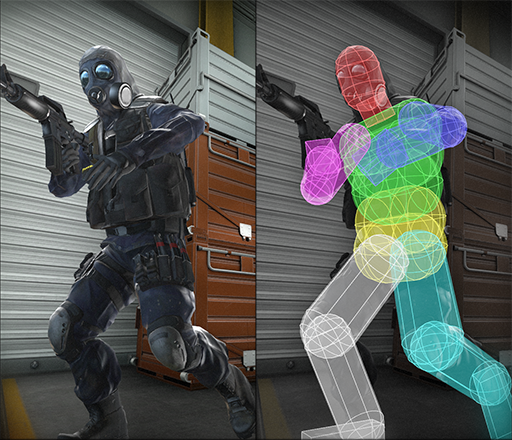
\includegraphics[width=1\textwidth]{./res/csgo_hitbox.png}
		\caption{Hitbox des Spieler-Modells aus dem Videospiel Counter Strike: Global Offensive; sichtbares Modell(links), mit eingeblendeter Hitbox (rechts)}
%%TODO source for pic
		\label{fig:chitbox}
	\end{subfigure}
~
	\begin{subfigure}[t]{0.2\textwidth}
		\centering
		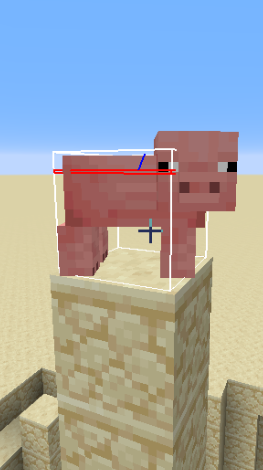
\includegraphics[width=1\textwidth]{./res/pig_hitbox.png}
		\caption{Hitbox eines NPC-Modells (Schwein) aus dem Videospiel Minecraft; Hitbox in weiß}
		\label{fig:mphitbox}
	\end{subfigure}
~
	\begin{subfigure}[t]{0.2\textwidth}
		\centering
		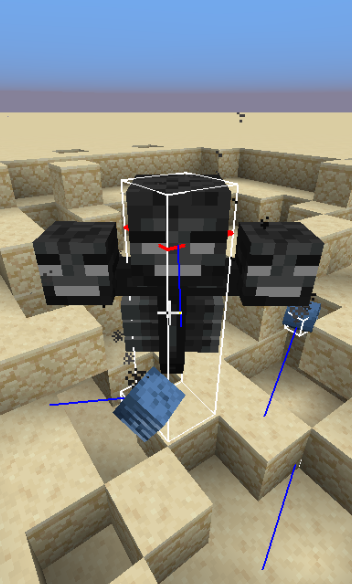
\includegraphics[width=1\textwidth]{./res/wither_hitbox.png}
		\caption{Hitbox eines NPC-Modells (Wither) aus dem Videospiel Minecraft; Hitbox in weiß}
		\label{fig:mwhitbox}
	\end{subfigure}

	\caption{Güten von Hitboxen}
	\label{fig:hitbox}
\end{figure*}

Die Abbildungen~\ref{fig:hitbox} zeigen Hitboxen in 2 verschiedenen Spielen.\\
\ref{fig:chitbox} zeigt das Spielermodell aus dem Spiel Counter-Strike: Global Offensive (CSGO). Links ist dabei das sichtbare Modell zu sehen, während rechts die Hitboxen eingeblendet sind. Die Hitboxen, welche hier nichmal mehr Boxen sind, sondern Ellipsoiden, decken das sichtbare Modell relativ genau ab. Ebenfalls zu erkennen ist die Partition in einzelne Hitboxen, zu sehen an den verschiedenen Farben der Hitboxen im rechten Bild.\\
Einzelne Details des Spielermodells, wie Riemen und Taschen an der Ausrüsung, sind nicht essentiell und werden daher auch physikalisch nicht abgebildet.\\
\ref{fig:mphitbox} und \ref{fig:mwhitbox} zeigen Hitboxen aus dem Spiel Minecraft bei zwei NPCs (Non-Player-Character (zu Deutsch: Nicht-Spieler-Charakter)). Es ist dort klar zu erkennen, dass die Hitboxen nicht sehr genau mit dem sichtbaren Modell übereinstimmen. Mehr noch: Die Minecraft-Hitboxen sind Koordinatenachsenparallel, d.h. Kanten verlaufen immer entlang der Koordinatenachsen der Raumrepräsentation.\\
Es wird versucht die Unterschiede zu rechtfertigen:\\
CSGO ist ein Shooter. Schnelle Reaktion und genaues Zielen sind ein hauptbestandteil des Produkts. Zudem ist CSGO ein hochkompetitiver E-Sport, der professionell gespielt wird. Es geht dabei um Preisgelder im siebenstelligen Bereich \cite{csgoprice}. Akkurate und, aus der perspektive des Spielers deterministische Hitboxen sind daher essenziell für das Produkt.\\
Die Partition der Hitboxen in CSGO ergibt sich direkt aus einer Anforderung der Anwendung, Schusstreffer auf verschiedene Teile des Spielermodells unterschiedlich zu bewerten. Beispielsweise verursacht der Treffer am Kopf am meisten Schaden. CSGO modelliert die unterschiedlichen Treffbaren teile des Modells also über mehrere Hitboxen.\\
Minecraft ist ein Sandbox Aufbauspiel. Ziel des Spiels ist der Bau von beliebigen Gebäuden, Tunneln, die Kreation von Maschinen oder das Erkunden von Gebieten.\\
In Minecraft steckt auch eine erhebliche Summe Geld. Am 15. September 2014 kaufte Microsoft die Entwicklerfirma und die rechte am Spiel für ca. 2,5 Milliarden Dollar \cite{buyminecraft}.\\
Das Kampfsystem in Minecraft forciert keine schnellen und genauen Treffer auf Gegner. Die gesamte Spielwelt ist aus sichtbaren Achsenparallel aufgestellten Würfeln gegeben, sind also Deckungsgleich mit entsprechenden achsenparallelen Hitboxen. Minecraft macht es sich einfach, da keine konkreten Anforderungen hinsichtlich Genauigkeit bestehen. Tatsächlich wird eine künstlich kleinere Hitbox manchmal sogar eingesetzt um einen Treffer zu erschweren (vgl. Abbildung \ref{fig::mwhitbox}).\\


\subsection{Hüllkörper}
Ein Bounding-Volume zu einem Objekt $o$ ist eine kompakte Menge $B_o \supset K_{o}$. $B_o$ kann als Hitbox fungieren.\\
Eine Bounding-Box ist ein spezielles Bounding-Volume in Form eines Quaders.\\
Eine in diesem Projekt extensiv verwendete, tiefere Spezialform der Bounding-Box ist die Axis-Alligned-Bounding-Box (AABB). Alle Kanten dieser Bounding-Box sind achsenparallel zu den Koordinatenachsen $\{(1,0,0), (0,1,0), (0,0,1)\}$ des 3D-Koordinatensystems.\\
Hier relevante Eigenschaften dieser sind:
\begin{itemize}
	\item kleine Datenrepresentation $AABB := (AABB_{o, min}, AABB) \in \mathcal{S}^{3^2}$ möglich.
		 In ihnen werden Minimal- und Maximalpositionen der AABB festgehalten.
	\item Schnelle Kollisionsüberprüfung zwischen AABBs durch Vergleiche der Extrema (Komplexität $= \mathcal{O}(1)$)
	\item Ermittlung einer minimalen AABB für ein Objekt durch Suche der Minima/Maxima (Komplexität $\le \mathcal{O}(n); n $ ist die Anzahl der Objektmerkmale (z.B. Ecken bei Polygon-Meshes))\\
		Die AABB muss sich an das eingeschlossene Objekt bei Bewegung anpassen. Standardmäßig durch Neuermittlung der AABB($\mathcal{O}(n)$). Optimierungen für verschiedene Arten von Bewegung möglich (Positionsänderung, Skalierung, etc.), aber manchmal schwierig (z.B. bei Rotation).
\end{itemize}

Im Falle des Spiels Minecraft werden AABBs als finale Hitboxen verwendet (vgl. \ref{fig:mwhitbox, fig:mphitbox}), welche jedoch scheinbar dem Kriterium $K_o \subseteq B_o$ zuwiderlaufen. Es muss an dieser Stelle zwischen der mathematischen Korrektheit einer Bounding-Box gegenüber einem gegebenen physikalischen Modell und der Designentscheidung gemacht werden, dass das sichtbare Modell nicht oder nur marginal die Grundlage des physikalischen Modells ist. In Minecraft ist die AABB die finale Hitbox  $H_{o, [min]} = K_o$ und definiert dadurch das Modell $K_o$. Das Bounding-Box-Kriterium ist damit theoretisch erfüllt. Die Designentscheidung selbst soll an dieser Stelle nicht eingeschätzt werden.




\section{Verwendungszwecke}
\label{sec:usages}
Kollisionsberechnung kann in Simulationen und im speziellen in Videospielen zu Realisierung vieler Features verwendet werden und wird daher in vielen verschiedenen Kontexten benötigt. 

Hinsichtlich der Menge von generell möglichen Anwendungen für Simulation sollen im Folgenden exemplarisch Anwendungsmöglichkeiten der Kollisionsermittlung aufgelistet werden, welche im Projekt von Relevanz sein können. Die Liste grenzt dabei auch den betrachteten Raum an Kontexten im Projekt auf ein überschaubares Maß ein. 

\begin{enumerate}
	\item logische Kollision\\
	\begin{enumerate}
		\item Anwesenheitsermittlung von Objekten\\
	Die Ermittlung der Anwesenheit von Objekten in einem bestimmten Teil des Raumes. Daraufhin können Eigenschaften der Objekte ermittelt werden, welche Auslöser für Ereignisse sein können oder Interaktionen unter Objekten können ausgelöst werden. Spezifischere Konzepte sind zum Beispiel: 
		\begin{enumerate}
			\item Raycasting\\
	Zur Ermittlung vom Objekt in Blickrichtung/Fokusobjekt oder Objekt am Cursor/Fadenkreuz wird ein Strahl in dieser Richtung mit Objekten kollidiert.\\
	Beispiel: Spieler möchte Tür öffnen, schaut Tür an, drückt Taste, Strahl ermittelt Tür in Blickrichtung und interpretiert Tastendruck als Tür-Öffnen-Befehl.
			\item Areale\\
	Objekte befinden sich in einem bestimmten Areal.
	Beispiel: In Stealth-Spielen werden zur Ermittlung, ob ein  Spieler sich im Sichtbereich eines Gegners befinden oft sogenannte View-Cones eingesetzt. Wie der Name suggeriert werden Entsprechende Berechnungen zur Sichtbarkeit des Spielers gegenüber dem Gegener ausgerechnet, sollte der Spieler mit der View-Cone des Gegners kollidieren
		\end{enumerate}
		\item Clipping\\
	Verhinderung, dass zwei Objekte in der Simulation den selben Raum einnehmen und miteinander verschmelzen, da dies bei typischen soliden Objekten nicht der Realität entspricht.
		\item Projektiltrefferermittlung
	\end{enumerate}

	\item Physikalische Kollision
		\begin{enumerate}
			\item Rigide Kollision\\
		Kollision von unzerstörbaren, unveränderlichen Objekten mit korrektem physikalischem Verhalten hinsichtlich Impuls.
			\item Zerstörung/Zerteilung von Objekten durch Kollision
		\end{enumerate}
\end{enumerate}

Es gibt viele weitere Anwendungen, welche durch die Verwendung von Kollisionsermittlung realisiert werden können, welche an dieser Stelle nicht weiter einbezogen werden sollen.



\section{Problemdefinition}
Kollisionserkennung (\textit{eng. collision detection}) ist die Erkennung der Überschneidung von zwei aus $k\in\mathbb{N}$ sich bewegenden Objekten in einem Raum.
Gesucht wird dabei der gezeitete Übergang vom Zustand der Nicht-Kollision zur Kollision.\\
Es gilt außerdem die Echtzeitanforderung (vgl.~Abschnitt \ref{sec:tick}).
\\
\subsection{Problemgrenzen}
Kollisionserkennung scheint, je nach Anwendungsfall, ein spezifisches Problem zu sein. Die anerkannte Terminologie für Kollisionserkennung scheint semantisch nicht eindeutig. Daher müssen für diese Studie klare Problemgrenzen und spezifische Begriffe definiert werden.\\
\\
Die erste Grenze ist temporal. Ein Tick (vgl.~Abschnitt \ref{sec:tick}) grenzt einen Simulationsschritt ein. Das Problem kann dabei auf die Abhandlung von einzelnen Simulationschritten beschränkt werden. Algorithmen müssen daher dynamisch bezüglich der Zeitgrenzen sein (Tickintervallgröße nicht konstant), diese dynamischen Grenzen aber nicht überschreiten können.\\
\\
Weiter werden verschiedene Level des Problems definiert:
\begin{itemize}
	\label{l0}
	\item[L0] Physikalische Repräsentation\\
		Überlegungen auf dieser Ebene behandelt die Auswahl möglicher mathematisch-technologischer Repräsentationen der Kollisionsphysik, welche wiederum Repräsentationen des Raums, der Zeit und der zu kollidierenden Objekte fordert.\\
		In dieser Studie wird sich damit nicht aktiv beschäftigt. Eine Repräsenation ist nötig und kommt daher passiv durch die Anforderungen der verwendeten Algorithmen und Technologien zu Stande.\\
			
	\label{l1}
	\item[L1] Suchraumfilter\\
		Annahme: Kollisionen finden zwischen Paaren von Objekten statt.
		Sei die Menge der Objekte im Raum $k\in\mathbb{N}$ so ist die Menge der Paare von Objekten, und damit die Menge möglicher Kollisionspaare, $k^2$.\\
		Bei naiver Überprüfung jedes Paares beträgt die Komplexität in dieser Ebene demnach $O(k^2)$ (vgl. \cite[Abschn. 2]{cd2D}).\\
		Verbesserungen dieser Komplexität können jedoch durch Vorfilterung des Suchraumes erreicht werden.\\
		Ziel ist dieses Levels ist es, eine Menge von Objektpaaren mit minimaler Anzahl von False-Positives zu ermitteln.

	\label{l2}
	\item[L2] Paarweise Kollisionserkennung\\
		Aus \ref{l1} vorliegende Objektepaare müssen auf tatsächliche Modellkollision Überprüft werden, da in L1 noch False-Positives enthalten sein können.
		Aus dieser genaueren Modellkollision können meist auch zusätzliche Informationen über die Kollision ermittelt werden (genaue Zeit, Ort, beteiligte Objektmerkmale), welche für die Kollisionsantwort benötigt werden.

	\label{l3}
	\item[L3] Kollisionsantwort/-auflösung\\
		In einer physikalischen Simulation hat eine Kollision meist eine physikalische Konsequenz, z.B. Geschwindigkeitsveränderung oder Verformung von Objekten. Die Konsequenz betrifft dabei nicht nur das beteiligte Objekt, sondern auch den gesamten Simulationsverlauf (z.B.~neue Kollisionsmöglichkeiten nach Kursänderung eines Objektes).\\
		Die L3-Schicht befasst sich mit der Umsetzung der Konsequenzen einer Kollision.
		Obwohl sich in dieser Arbeit mit den Konsequenzen der Kollision eigentlich nicht beschäftigt werden soll, muss hierzu ein Kontext hergestellt werden, vor allem um Anforderungen an andere Schichten zu ermitteln.
\end{itemize}





\section{L1 : Suchraumverkleinerung/Kollisionspaarermittlung}
Da die exakte Berechnung einer Kollision signifikant viel Rechenleistung benötigt, ist eine Vorfilterung sinnvoll. Diese schließt einen Großteil der Objektpaare schon vorher aus. Eine Kollision kann z.B. nur dann passieren, wenn die Hüllobjekte der beiden Objekte ebenfalls kollidieren (wegen der Eigenschaft //TODO mathe). Hier wird als Hüllobjekt eine AABB verwendet. Bestimmte Arten der logischen Kollision benötigen außerdem keine genauere Berechnung, sodass die verbleibenden Objektpaare nach der Vorfilterung direkt eine logische Kollision eingehen. Um verschiedene Arten der Kollision behandeln zu können und die Objektpaare dem richtigen Algorithmus für die nächste Stufe zuführen zu können, wurde im Rahmen des Projekts eine Komponente erstellt, die dieses Problem mit austauschbarem Vorfilterungsalgorithmus löst. (Ungenügende Ansätze der Behandlung verschiedener Kollisionstypen unter Verwendung eines nicht austauschbaren Vorfilterungsalgorithmus haben schon vor dem Projektstart in der Codebasis existiert). \\
Logische und physikalische Kollisionen werden als (lokale) Interaktionen zusammengefasst und werden in 2 Kategorien eingeteilt:
//TODO format
1. Symmetrische Interaktionen: Beide Objekte des Objektpaares gehören der selben Klasse an (z.B: die Kollision rigider Objekte, wie sie in //TODO ref beschrieben wird).
2. Asymmetrische Interaktionen: Objektpaare setzen sich aus 2 Objekten verschiedener Klassen zusammen (z.B. Projektil und treffbares Objekt). Kollisionen innerhalb des selben Objekts treten hier nicht auf (Projektile interagieen nicht mit anderen Projektilen).

In jeder Kategorie können mehrere Interaktionstypen enthalten sein. Jeder Typ wird hier einzeln betrachtet und ihm kann so ein eigener Vorfilterungsalgorithmus zugewiesen werden, der entsprechend zugeschnitten und problemspezifisch optimiert werden kann.
Die Aufgabe des Vorfilterungsalgorithmus unterscheidet sich je nach Kategorie der Interaktion etwas:
//TODO format
1. Symmetrische Interaktionen: Aus Menge aus n Objekten werden alle diejenigen (maximal n²) Objektpaare ausgewählt, deren AABBs sich überschneiden. Als untere Schranke kann man Omega(n+i) angeben, wobei i die Anzahl der tatsächlichen Überschneidungen ist. Die obere Schranke O(n²) erhält man durch naives Ausprobieren jeder Kombination.
2. Asymmetrische Interaktionen: Aus 2 Mengen von n und m Objekten werden alle diejenigen Objektpaare mit jeweils einem Mitglied aus jeder Menge ausgewählt, deren AABBs sich überschneiden. Als untere Schranke kann man Omega(n+m+i) angeben. Die obere Schranke O(n*m) erhält man durch naives Ausprobieren jeder Kombination.

Für die Laufzeit bei praktischen Problemen sei angemerkt, dass die Konstante oft eben so wichtig zu betrachten ist wie die asymptotische Komplexität. \\

Im folgenden werden 2 Algorithmen, die im Rahmen des Projekts implementiert wurden, näher beschrieben.

//TODO format
1. Boxsort
//TODO

//TODO format
2. Spatial Hashing
Die Grundidee besteht hier dabei, den Raum in viele Bereiche (sog. chunks) aufzuteilen und Kollisionspaare nur innerhalb dieser Bereiche zu suchen. Sind 2 Objekte weit voneinander entfernt und somit nicht im selben chunk, ist eine Überschneidung der AABBs nicht möglich und muss deshalb auch nicht betrachtet werden. Ein Beispiel für 2 Dimensionen sieht man in Abb.~\ref{fig:spatialHashing}.

\begin{figure}
    \centering
    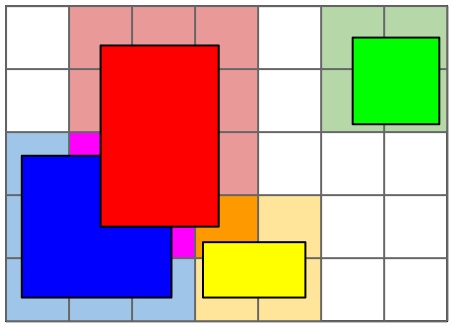
\includegraphics[width=0.5\textwidth]{./res/spatialHashingAABB.png}
    \caption{2D-Beispiel von Spatial Hashing von AABBs (stark gefärbte Rechtecke). Die leicht gefärbten Bereiche sind chunks, die ein Objekt der entsprechenden Farbe(n) beinhalten.}
    \label{fig:spatialHashing}
\end{figure}

Man sieht in Abb.~\ref{fig:spatialHashing}, dass Objekte mit mehreren chunks überlappen können. Ein Objekt muss sich in jedem chunk anmelden, das sich mit seiner AABB überschneidet, zu sehen z.B. beim grünen Objekt, das sich in den 4 chunks rechts oben anmelden muss. Gibt es keine weiteren Objekte in den chunks, wo sich das Objekt angemeldet hat, müssen keine potentiellen Kollisionen berechnet werden. Ist dies für alle Objekte der Fall, ist die optimale Komplexität O(n) im symmetrischen Fall erreicht (bei konstanter Maximalgröße von Objekten). Im asymmetrischen Fall können mehrere Objekte im selben chunk angemeldet sein, ohne dass eine Kollision auftritt, solange die Objekte alle vom selben Typ sind. In diesem Fall ist die optimale Komplexität von O(n+m) im asymmetrischen Fall erreicht (bei konstanter Maximalgröße von Objekten). \\
Werden mehrere Objekte, die für eine Kollision kompatibel sind, in einem chunk angemeldet, so müssen alle potentiellen Kollisionspaare überprüft werden (hier mit naivem //TODO Mathe O(n²) bzw. O(n*m) Algorithmus). Die Überprüfung kann entweder direkt bei der Anmeldung erfolgen (hier implementiert) oder erst nach Eintragung aller Objekte erfolgen, was die Auswahl an für die weitere Auflösung verwendbaren Algorithmen erhöht. \\
Ein potentielles Problem kann in Abb.~\ref{fig:spatialHashing} bei der Überschneidung des roten und blauen Objekts betrachtet werden. Erfolgt eine Überlappung in mehreren chunks, besteht die Gefahr der mehrfachen Behandlung von Kollisionen. Deshalb wird während der Partnerfindung ein Hashtable mit schon behandelten Objekten mitgeführt, womit effizient Duplikate vermieden werden. Auf diese Maßnahme kann verzichtet werden, wenn sich das Objekt nur in einem chunk befindet.\\
Um das Anlegen vieler leerer chunks zu vermeiden und trotzdem schnellen Zugriff zu haben, wird ein Hashtable zur Verwaltung der chunks verwendet. Dazu wurde eine passende Hashfunktion gesucht und eingebunden, die plattformunabhängig aber dennoch mit sehr geringer Laufzeit $HASH: \mathcal{I}^3 \mapsto \mathcal{I}_{64}$ mit $\mathcal{I}_{64}$ als 64-Bit Integer einem Hashwert zuordnet. $i: (i, f)\in\mathcal{S}$
\section{Paarweise Modellkollisionen}
\label{sec:l2}
Die paarweise Kollisionserkennung bezieht sich auf die Kollision von konkret zwei 3D-Modellen. In diesem Schritt ist die Genauigkeit der Kollision bei steigender Modellkomplexität im Fokus.
Ziel ist es die Diskrepanzen zwischen der grafischen Anzeige von Modellen und der physikalischen Simulation zu deckeln.
\subsection{Input}
Aus dem vorhergehenden Schritt der Kollisionspaarermittlung werden für den Schritt der paarweisen Kollisionserkennung bis zu  $|OBJ|^2$ Objektpaare $C_{guess}\subseteq OBJ^2$ erhalten, für die eine Kollisionsvermutung während eines Ticks gilt. Man geht weiter davon aus, dass die Menge der tatsächlichen Kollisionen $C_{definitive}\subseteq OBJ^2$ in der Menge der vermuteten Kollisionspaare  vollständig enthalten ist $C_{definitive}\subseteq C_{guess}$, d.h. keine tatsächlichen Kollisionspaare im Paarermittlungsprozess verloren gehen. 

\subsection{Output}
Es ist eine Aufgabe dieses Schritts, die Reduzierung von $C_{guess}$ auf $C_{defintive}$ zu vollenden.\\
Eine zweite Aufgabe ist die Ermittlung von Informationen über den Hergang der Kollisionen der Paare in $C_{defintive}$.
Im Abschnitt~\ref{sec:usages} werden einige Verwendungszwecke der Kollisionsermittlung aufgelistet. 
Elemente der Aufzählung haben unterschiedliche Anforderungen hinsichtlich benötigter Information über den Kollisionsvorgang um realisiert werden zu können.

\begin{enumerate}
	\item Schnitt\\
		Die Frage ob Objekte $o_0,o_1 \in OBJ$ sich an einem konkreten Zeitpunkt während eines Ticks $t\in \Upsilon_{\delta i}$ schneiden/gegenseitig enthalten. $K_{o_0, t} \cap K_{o_1, t} \neq \emptyset$.
	\item Intrusion\\
		Die Frage nach den Eigenschaften
		\begin{enumerate}
		\item ob
		\item wann
		\item an welcher Raumposition
		\item mit welchen Teilen des Objektes
		\end{enumerate}
		ein Eindringen eines Objektes in ein anderes stattfindet, d.h. ein Zustandsübergang von Nicht-Kollision zu Kollision stattfindet.
		Der durchsuchte Zeitraum ist dabei eine kontinuierliche Schlusspartition der Ticksequenz $\Upsilon_{part} = \langle t_{searchstart}, ..., t_1 \rangle : (\Upsilon_{\delta i}\backslash \Upsilon_{part}) \smallfrown \Upsilon_{part} = \Upsilon_{\delta i} $ ($\smallfrown$ ist Konkatenation von Sequenzen) zu der relativ bei Zeitpunkt $j \in \Upsilon_{part} \subseteq \Upsilon_{\delta i}$ eine Erstkollision auftritt.\\
		So können nach dem finden der Erstkollision prinzipiell durch das verschieben von $t_{searchstart}$ noch weitere Erstkollisionen während des Ticks $\delta_i$ ermittelt werden.
		$$\exists j \in [1, |\Upsilon_{part}|-1], t_c= \Upsilon_{part}(j):$$
		$$ G_{o_0, t_c}\cap G_{o_1, t_c} \neq \emptyset \wedge \forall j' < j: 
		G_{o_0, \Upsilon_{part}(j')}\cap G_{o_1, \Upsilon_{part}(j')} = \emptyset$$
		Aus der Schnittmenge $G_{o_0, t_c}\cap G_{o_1, t_c}$ können dann die Angeforderten Eigenschaften zur Kollision (Zeit, Ort, Beteiligte Objektteile) ermittelt werden.
\end{enumerate}
Es mag weitere Forderungen an Kollisionsalgorithmen geben. Die obige Aufzählung stellt dabei die in dieser Arbeit in Betracht gezogenen dar.

Für physikalische Verwendungszwecke insbesondere bei der rigiden Objektkollision erscheint Intrusion besonders interessant. In Simulationen mit rigiden Kollisionsobjekten ist typischerweise der Zustand des Schnitts zweier Objekte nicht erlaubt und muss daher aktiv durch eine Kollisionsreaktion verhindert werden. Durch die Ermittlung des ersten Zeitpunkts des Bruchs der Nicht-Überschneidungsbedingung kann die Kollisionsreaktion passend ermittelt werden.\\
Die Umsetzung der Auflösung von Kollisionen und Mehrfachkollisionen ist explizit aus diesem Projekt ausgeschlossen. Selbst jedoch bei der theoretischen Betrachtung von Mehrfachkollisionen während eines Ticks und Optionen zu deren Auflösung, bzw.~physikalischer Reaktion von Objekten , scheinen vorwiegend Erstkollisionen interessant zu sein.\\
An dieser Stelle wird demnach die Annahme getroffen, dass zunächst nur Erstkollisionen durch Intrusion interessanter sind sind und zuerst ermittelbar gemacht werden sollten.


%%TODO look if one can fit that under his hat somewhere, would be rad 
%Ein interessanter Fehler bezogen auf L3 in freier Wildbahn ist in \cite{skyrimwallglitch} zu sehen. Es handelt sich dabei um einen Glitch im Spiel The Elder Scrolls V:Skyrim. Dabei wird eine gleichzeitige Kollision des Spielermodells (welches sich durch eine Ingame-Fähigkeit unüblich schnell bewegt), eines Objekts und einer Wand oder Tür provoziert. Die Kollision, bzw. die wiederholten Kollisionen zwischen dem Spielermodell, dem Objekt (Kessel/Teller/Korb) und der Wand/Tür werden nicht richtig aufgelöst, was dazu führt, dass der Spieler durch die Wand laufen kann.\\


\subsection{Intrusionsermittlung durch lineare Interpolation der Objektbewegung}
\label{sec:linear_int}
Um das Problem zu vereinfachen wird die zunächst die Rotation von Objekten vernachlässigt.\\
Genauer: In diesem Kontext erfährt ein Objekt $o\in OBJ$ während eines Ticks $\delta_i$ keine zeitliche Änderung der Rotation $\forall t \in \Upsilon_{\delta i} : \omega(o, t) = (0,0,0)$. Dies hat mehrere Gründe:
\begin{enumerate}
\item Objekte hielten zum Start des Projekts noch keine Repräsentation für Rotation.
\item Rotation mit einzubeziehen wurde zu Anfang schon als schwierig eingestuft. Dieser Verhalt sollte sich später bestätigen.
\item Es gibt genügend Kollisionsszenarien/Verwendungszwecke für denen Rotation keine Rolle spielen muss. (Logische Kollision, punktförmige Objekte, unbewegliche Objekte wie z.B. oft Terrain, Verwendungszwecke mit hoher Fehlertoleranz)
\item Es wird ein Experiment der Vernachlässigung von Rotation durchgeführt. Es soll dabei beantwortet werden, ob auch ohne Behandlung der Rotation eine ausreichend zufriedenstellende Illusion von physikalischem Realismus geschaffen werden kann.
\end{enumerate}

Wie in Abschnitt~\ref{sec:objects_sim} bereits beschrieben sind die zeitlichen Änderungen (Geschwindigkeit $v$ und Drehgeschwindigkeit $\omega$) eines Objektes während eines Ticks konstant. Durch die Vernachlässigung der Drehgeschwindigkeit $\omega$ kann die zeitliche Änderung eines Objektes $o$ allein auf Bezug zu Geschwindigkeit $v$ und der Zeit $t$ beschrieben werden, bzw.~alle im Objekt $o$ enthaltenen Punkte $p \in G_o$ beschreiben lineare, parallele Flugbahnen während des Ticks $\delta_i$:
$$l_p = \{p + (t - t_0) * v(o, t_0) | t_0 \leq t \leq t_1\}$$
%%; X \subseteq \mathcal{F}^3:\{l_p|p\in X\} = \{X| t \in \Upsilon_{\delta_i}\}$$
In ihrer Gesamtheit beschreiben diese das durchlaufene Volumen des Objekts:
$$\{l_p|p\in G_o\} = \{G_{o, t}| t \in \Upsilon_{\delta_i}\}$$

Dies ermöglicht die Ermittlung von Kollisionen von Objekten $o_0, o_1$ durch lineare Interpolation der Zeit.\\
Die Eigenschaft der Linearität hat dabei noch den weiteren entscheidenden Vorteil, dass bei einer Relativierung der Objekte wechselseitig zueinander, eine Operation der einer Transformation in Form einer Translation gleichkommt, die Linearität weiterhin gewahrt bleibt. Zum Vergleich: Mit aktiver Rotation beschreiben Objekte relativ zueinander Kurvenflugbahnen.\\
Essenziell zu überprüfende Merkmalspaare $\in \{Area, Edge, Vertex\}^2$ sind:
%TODO formatting clips left
		\begin{itemize}
			\item [$\{Vertex, Area\}$] Eine Ecke durchschlägt eine Fläche.\\
				$\Rightarrow$ Zu überprüfende Paare: $(V_{o_0}\times A_{o_1})\times (V_{o_1}\times A_{o_0})$
			\item [$\{Edge, Edge\}$] Kanten durchschneiden sich gegenseitig.
				$\Rightarrow$ Zu überprüfende Paare: $(E_{o_0}\times E_{o_1})\times (E_{o_1}\times E_{o_0}) = (E_{o_0}\times E_{o_1})$
		\end{itemize}
		Alle anderen Kombinationen sind entweder in diesen beiden enthalten (z.B. $\{Vertex, Edge\}$ in 1.) oder ein Ereignis dieser beiden Szenarien muss logisch vorher passieren (z.B. 1. oder 2. muss vor $\{Edge, Area\}$ bereits passiert sein).
\ \\
		Aufgrund der Relativierung muss nur eines der Merkmale eine zeitliche Bewegung durchführen.
		\begin{itemize}
			\item [$$\{Vertex, Area\}$$] 2 Möglichkeiten:
				\begin{itemize}
					\item[Option 0:] Eckpunkt $v \Rightarrow$ Linie $l_v$
					\item[Option 1:] Dreiecksfläche $a \Rightarrow$ Schiefes Prisma $ \{l_p | p \in \mathcal{A}(a)\}$
				\end{itemize}
				Gewählt wird Option 0, da einfachere Berechnung.
			\item [$\{Edge, Edge\}$] Kante $e \Rightarrow$ Parallelogramm $\{l_p | p \in \mathcal{E}(e)\}$
		\end{itemize}
\ \\
		Geometrische Eigenschaften nun beteiligter Formen:
		\begin{itemize}
			\item [Linie] $L = \{p_l | x\in\mathcal{F} ; p_{l0}, p_{l1} \in \mathcal{F}^3 ; p_l = p_{l0} + x * p_{l1}; 0\le x\le 1 \}$
		\item [Dreieck] $T = \{p_t | x,y \in\mathcal{F};  p_{t0},  p_{t1},  p_{t2} \in \mathcal{F}^3; p_t = p_{t0} + x*p_{t1} + y*p_{t2}; 0\le (x+y) \le 1\}$
			\item [Parallelogramm] $P = \{p_p | x,y \in\mathcal{F}; p_{p0}, p_{p1}, p_{p2} \in \mathcal{F}^3; p_p = p_{p0} + x*p_{p1} + y*p_{p2}; 0\le x\le 1; 0\le y\le 1\}$
		\end{itemize}
\ \\
		Beide Szenarien können über Gleichungssysteme zur Ermittlung von Ort- und Zeitkoeffizienten in konstanter Zeit überprüft werden:
		\begin{itemize}
			\item [$\{Vertex, Area\}$] $p_{l0} + x * p_{l1} = p_{t0} + y*p_{t1} + z*p_{t2}$\\
				$x$ ist zudem hier der Koeffizient der Zeit, da die Linie in der Zeitdimension liegt.
			\item [$\{Edge, Edge\}$] $p_{l0} + x * p_{l1} =  p_{p0} + y*p_{p1} + z*p_{p2}$\\
				Sei die ursprüngliche Kante, aus dem das Parallelogramm generiert wurde $\{p_0+y*p_1\}$, so liegt die andere Kante $\{p_0 + z*p_2\}$ in der Zeitdimension und somit ist hier z der Zeitkoeffizient.
		\end{itemize}
\ \\
		Komplexität: $\mathcal{O}(|V_{o0}|* |A_{o1}| + |V_{o1}|*|A_{o0}|$ + $|E_{o0}| * |E_{o1}|)$

		\begin{itemize}
			\item Zuverlässige Ermittlung der Erstkollision durch Findung des minimalen Zeitkoeffizienten.
			\item Mathematisch exakte Ermittlung der Zeit einer Kollision durch Zeitkoeffizienten.
			\item Mathematisch exakte Ermittlung des Orts einer Kollision durch Ortskoeffizienten.
			\item Ermittlung der Beteiligen Objektmerkmale der Erstkollision.
		\end{itemize}
Wie beschrieben kann dieses Verfahren bereits in einigen Szenarien, bei denen Rotation keine Rolle spielt, als vollständige Lösung zum Einsatz gebracht werden.\\
Es bleibt das Experiment, eine Illusion physikalischer Vorgänge mit rigider Körperkollision über den Linearen-Interpolationsalgorithmus zu realisieren.\\
Zunächst scheint dabei klar: Durch die Vernachlässigung der Rotation passieren physikungetreue Fehler, besonders, je größer die Varianz des Abstands der vom Objekt enthaltenen Punkte zum Objektursprung ist. Objekte sind dann unförmig und durchstreifen bei zeitlicher Bewegung logisch ein zu einem gewissen Grad anderes Volumen, als der lineare Interpolationsalgorithmus annimmt. Diese Diskrepanz kann sowohl zu False-Positives als auch zu False-Negatives führen.\\
Des Weiteren muss die vernachlässigte Rotation nachgeholt werden. Durch einen Extremfall dieser Nachlässigkeit fällt ein weiteres Defizit des Algorithmus auf. Ist die relative Geschwindigkeit zweier Objekte $=0$, wird aus Sicht des Algorithmus' kein Volumen durchstreift. Es werden zwischen diesen Objekten dann gar keine Kollisionen erkannt, welche durch Rotation logisch/visuell aber auftreten.\\
Man versucht diese Problem durch statische Kollisionstests am Tickende zu lösen. Dabei wird die akkumulierte Rotationsbewegung/Rotationstransformation auf einmal ausgeführt. Vor und nach der Bewegung wird statisch eine Kollisionsabfrage berechnet.\\
Diese Anpassung bringt eigene Probleme mit sich:
\begin{enumerate}
\item Durch die akkumulierte Drehung kann eine Kollision bei schnellen Drehgeschwindigkeiten durch nur die Tests am Anfang und am Ende des Ticks komplett übersehen werden.
\item Nach der Rotationstransformation können Objekte sich in einem gegenseitigen Schnittzustand $D(o_0, t_1)\cap D(o_1, t_1) \neq \emptyset$ befinden, da an dieser Stelle keine Intrusion erkannt werden kann. Der Zustand könnte durch einen Linearen-Interpolationsalgorithmus zwar erkannt werden, jedoch sind bis dato im Projekt keine Möglichkeiten enthalten, vernünftig auf diesen Fall zu reagieren.
Eine Idee ist die Suche nach einem Zeitpunkt vor der Überschneidung, durch beispielsweise Bisektion (binäre Suche) des Drehungsausschlags. Es erscheint jedoch, dass der wiederholte Aufwand durch Transformation und Ausführen des Interpolationsalgorithmus in der gegebenen Zeit ebenfalls keine qualitativ hochwertigen Ergebnisse erzielt. Der Schnittzustand wird zudem in der rigiden Körperkollision als fehlerhafter Zustand angesehen, den die Kollisionsroutine eigentlich verhindern soll.
\end{enumerate}

%%TODO glitchpic

Es wird also weiter nach Lösungen gesucht, die sich dem Rotationsproblem besser annehmen.

\subsection{Gilbert-Johnson-Keerthi-Distanzalgorithmus (GJK)}
\label{sec:gjk}

\begin{figure}
\centering
\begin{tikzpicture}

\draw (-3.5,-2.5) rectangle (4.5,2.5);
\draw[thick,->] (-3.5,-2.5) -- (4.5,-2.5) node[anchor=south east] {X};
\draw[thick,->] (-3.5,-2.5) -- (-3.5,2.5) node[anchor=north west] {Y};


\coordinate (O) at (0,0) ;
\draw [below](O) node[black]{$O$};
\draw (O) node[black]{\textbullet};

\coordinate (Ta) at (3, 0);
\coordinate (Tb) at (4, 1);
\coordinate (Tc) at (4, -1);

\draw[red] (Ta) -- node[above left]{$G_{o_1}$} (Tb) -- (Tc) -- cycle; 

\coordinate (Qa) at (1, -1);
\coordinate (Qb) at (1, 1);
\coordinate (Qc) at (2, 1);
\coordinate (Qd) at (2, -1);

\draw[blue] (Qa) -- (Qb) -- node[above]{$G_{o_0}$} (Qc) -- (Qd) -- cycle; 

\coordinate (QaTa) at (-2, -1);
\coordinate (QbTa) at (-2, 1);
\coordinate (QcTa) at (-1, 1);
\coordinate (QdTa) at (-1, -1);
\coordinate (QaTb) at (-3, -2);
\coordinate (QbTb) at (-3, 0);
\coordinate (QcTb) at (-2, 0);
\coordinate (QdTb) at (-2, -2);
\coordinate (QaTc) at (-3, 0);
\coordinate (QbTc) at (-3, 2);
\coordinate (QcTc) at (-2, 2);
\coordinate (QdTc) at (-2, -0);

\draw[red] (QaTa) -- (QaTb) -- (QaTc) -- cycle; 
\draw[red] (QbTa) -- (QbTb) -- (QbTc) --  cycle; 
\draw[red] (QcTa) -- (QcTb) -- (QcTc) -- cycle;
\draw[red] (QdTa) -- (QdTb) -- (QdTc) -- cycle;

\draw[blue] (QaTa) -- (QbTa) -- (QcTa) -- (QdTa) -- cycle; 
\draw[blue] (QaTb) -- (QbTb) -- (QcTb) -- (QdTb) -- cycle; 
\draw[blue] (QaTc) -- (QbTc) -- (QcTc) -- (QdTc) -- cycle; 

\node at (-1.8, 1.5)[above right]{$\mathcal{M}(G_{o_0}, G_{o_1})$};

\end{tikzpicture}
\caption{2D-Beispiel für eine Minkowski-Differenz $\mathcal{M}(G_{o_0}, G_{o_1})$ mit Ursprung $O$ und den als Mesh angegebenen Objekten $G_{o_0}$ und $G_{o_1}$. Gezeigte Linien dienen als Hilfestellung zur Erkennung von Einflüssen der Ursprungsobjekte auf die Differenz.}
\label{fig:gjk}
\end{figure}
GJK ist ein Algorithmus, der zwischen kompakten, konvexen Mengen $K_0, K_1 \subseteq \mathbb{R}^3$ die minimale euklidische Distanz $distance(K_0, K_1) = min\{|k_0 - k_1|~| k_0\in K_0 ; k_1 \in K_1\}$ errechnet. Er wurde 1988 publiziert \cite{gjk} und scheint heute gerne in Videospielen verwendet zu werden. Beispiele sind dabei Blizzard Entertainments Diabolo 3 \cite{gdc-physics} und Valves Half-Life 2\cite{gjk-casey}.\\
Die Urquelle \cite{gjk} beschreibt den Algorithmus umfassend mathematisch und detailliert. Es wird weiter Quellmaterial \cite{gjk-casey} mit praktischem Fokus zu Rate gezogen, um eine Implementierung umzusetzen und den Einstieg zu erleichtern.
Im GJK-Algorithmus sollen Eigenschaften der sogenannten Minkowski-Differenz $\mathcal{M}:\mathcal{P}(\mathbb{R}^3)^2\mapsto \mathcal{P}(\mathbb{R}^3); \mathcal{M}(K_0, K_1) = \{a - b| a\in K_0 ; b\in K_1\}$ \cite[p.195]{gjk} ausgenutzt werden.
Ein Beispiel für die Minkowski-Differenz ist in Abbildung \ref{fig:gjk} zu sehen. Die hier relevanten Eigenschaften der Minkowski-Differenz lauten wie folgt:\\
	\begin{enumerate}
		\item Die Minkowski-Differenz zweier konvexer Körper ist ebenfalls konvex \cite[p.195]{gjk}.
		\item Spezielle Eigenschaften bezüglich Distanzen und Schnitt der Ursprungsobjekte:
		\begin{enumerate}
			\item $K_0 \cap K_1 \neq \emptyset \Rightarrow \exists a_o, b_o \in K_0 \cap K_1, a_0 \in K_0, b_0 \in K_1 : a_o = b_o \Rightarrow a_o - b_o = O \Rightarrow O \in \mathcal{M}(K_0, K_1)$
			\item $K_0 \cap K_1 = \emptyset \Rightarrow \forall a_o\in K_0, \forall b_o\in K_1 : a_o \neq b_o \Rightarrow a_o - b_o \neq O \Rightarrow O \notin \mathcal{M}(K_0, K_1)$.
			\item $distance(O, \mathcal{M}(K_0, K_1)) = distance(K_0, K_1)$
			\item (2a.) $\wedge$ (2b.) $\wedge$ (2c.) $\Rightarrow K_0 \cap K_1 \neq \emptyset \Leftrightarrow O \in \mathcal{M}(K_0, K_1)	\Leftrightarrow distance(K_0, K_1) = 0$
		\end{enumerate}
		\item (2c.) $\Rightarrow distance: \mathcal{P}(\mathbb{R}^3)^2 \mapsto \mathbb{R}^+_0$ (gibt nur positive Distanzen aus)
	\end{enumerate}
Durch die Eigenschaften der Minkowski-Differenz wird, im Gegensatz zum vorigen Verfahren in Abschnitt \ref{sec:linear_int} das Schnittproblem statt des Intrusionsproblems behandelt.
Durch die Fähigkeit des GJK-Algorithmus, die Distanz zwischen zwei Objekten zu ermitteln, ist dieser jedoch ein praktisches Werkzeug, um das Intrusionsproblem ebenfalls zu lösen.
Zum Beispiel ist ein Ansatz mit GJK, durch Abstraktion über einer Nullstellensuche der Distanz zwischen zwei Objekten das Intrusionsproblem abzubilden (vgl.~Eigenschaft 2d, vgl. \cite{gdc-physics}).\\
GJK eignet sich also für dieses Projekt und soll implementiert werden. 

Zunächst muss die Eingabeinformation von kompakten, konvexen Punktmengen, die der Algorithmus fordert, äquivalent hergestellt sein, um sicherzustellen, dass der Algorithmus auch mit Polygon-Meshes durchgeführt werden kann. Für diese ist allerdings keine Konvexität gefordert und eine entsprechende kompakte Repräsentation nicht gegeben.
Zunächst soll Konvexität hergestellt werden. Definierte nicht-konvexe Objekte können in konvexe Partitionen aufgeteilt werden. Jede Partition zählt dann als eigenes Objekt gegenüber dem Algorithmus. Das erhöht die erwartete Komplexität der gesamten Kollisionsroutine mit GJK um den Grad der Partitionierung ($\mathcal{O}(|P_{o_0}|*|P_{o_1}|)$).\\
\ \\
Es wurde zu einer automatisierten Methode recherchiert, um die Partitionierung herzustellen. Insbesondere die minimale Partitionierung scheint hier von Interesse, um die Erhöhung der Komplexität zu mitigieren.\\
Zusätzlich zu eigenen Überlegungen bestätigen die Quellen \cite{ARTIGAS20111968} und \cite{grelier2019minimum} die NP-Vollständigkeit, bzw. NP-Härte zusammengehöriger Probleme der minimalen konvexen Partitionierung.\\
Eine nicht minimale Partitionierung wäre zunächst auch ausreichend und auch lange Berechnungszeiten zur Partitionierung würden für rigide Objekte nur einmaligen Aufwand zum Programmstart bedeuten und wären daher nicht kritisch.\\
Bei Versuchen, Algorithmen für dieses Problem zu erstellen, wird jedoch eine weiter klare Hürde erkenntlich: Allein durch die Polygon-Mesh, sind Innen und Außenseite des Objektes prinzipiell nicht definiert.\\
Für grafische Zwecke kann dieser Bezug oft durch das sog. \textit{Winding} eines Dreiecks angegeben werden. Dabei wird die Reihenfolge der Angabe der Ecken eines Dreiecks konventionell festgelegt, wodurch die Richtung der Flächennormale eines Dreiecks kontrolliert werden kann, die dann Außen oder Innenseite spezifiziert. Auch die direkte Angabe einer Flächennormale zu jedem Dreieck (oder sogar jedem Eckpunkt) is im graphischen Kontext für bestimmte Effekte gebräuchlich. Diese Konzepte werden grafisch im Projekt jedoch bis dato nicht verwendet und sind daher auch nicht vorhanden.\\
Eine Konvention für ein \textit{Winding} wurde allerdings im Projekt eingeführt, nicht zuletzt, da diese die Implementierung des GJK vereinfacht.\\
Für die in dieser Projektarbeit verwendeten Testzwecke erscheint der Aufwand der Automatisierung der konvexen Partitionierung für dieses Projekt letztendlich doch zu hoch und thematisch zu fremd.\\
\ \\
Die konvexe Partitionierung des Objektes $o$ wird daher manuell und explizit bei Modellen durch die Angabe von Mengen von Indices von zueinander konvexen Eckpunkten $P_o := \{P_0, ...\}; P_i \subseteq V_o$ angegeben.\\
Zusätzlich ist die Äquivalenz zur kompakten Punktemenge $K_o$ gefordert. Diese ist nun implizit durch die Konvexität gegeben. $K_o$ ist konvex, wenn gilt $\forall p_0, p_1 \in K_o, \forall x \in [0,1] : p0 + x * (p_1 - p0) \in K_o $. In Mesh-Repräsentation $G_o$ sind nicht alle diese Punkte enthalten. Jedoch, wenn $K_o$ konvex, so sind die Hüllen $\mathcal{H}(K_o) = G_o$ ebenfalls konvex. Alle Punkte $K_o \backslash G_o$ können so durch die Konvexitätsdefinition impliziert werden. Die zusätzlich mit der Objektrepräsentation mitgelieferte Partitionierung erweitert also die verfügbare Information und schafft in dieser Hinsicht Äquivalenz zwischen Polygon-Meshes und kompakten Mengen und die Unterscheidung von Innen und Außen. Informationen zu verbundenen Ecken einer Polygon-Mesh $I_o$ werden dadurch in diesem Kontext ebenfalls redundant. Der Algorithmus kann demnach außschließlich unter Einbeziehung von Eckpunkten $V_o$ und der Partitionierung verfahren.\\
Durch die Feststellung der Äquivalenz wurde ermittelt, dass eine Variante des GJK-Algorithmus auch an Polygon-Meshes durchgeführt werden kann.\\
Es kann also eine Diskretisierung/Beschränkung auf die Information der Eckpunkte der Polygon-Mesh $V_o$  verwendet werden, was vorteilhafte Iterationslängen im Algorithmus zur Folge hat ($V_o \ll G_o \ll K_o$).\\
Eigenschaften der Minkowski-Differenz müssen den Umstand der Diskretion respektierend ausgenutzt werden.\\

\begin{enumerate}
		\item Die diskrete Minkowski-Differenz ist ebenfalls konvex.	
		\item Ein Simplex ist eine durch eine Anzahl $n\in\mathbb{N}$ Eckpunkte $s\in\mathcal{M}(V_{o_0}, V_{o_1})^n$ aufgespannte $n$-dimensionale geometrische, inhärent konvexe Form (hier: Punkt für $n=1$, Gerade $n=2$, Dreieck $n=3$, Tetraeder $n=4$). Durch die Konvexität ist die entsprechende kompakte Menge $K_s$ implizit definiert.
		\item Für das nächste Simplex $s_{nearest} \in \mathcal{M}(V_{o_0}, V_{o_1})$ zum Ursprung $O$ gilt außerdem $distance(O, s_{nearest}) = distance(K_{o_0}, K_{o_1})$ \cite[p. 195]{gjk}. 
		\item $O \in \mathcal{M}(K_{o_0}, K_{o_1}) \nRightarrow O \in \mathcal{M}(V_{o_0}, V_{o_1})$. Jedoch kann eine äquivalente Beziehung gefunden werden: $O \in \mathcal{M}(K_{o_0}, K_{o_1}) \equiv \exists Simplex~s \in \mathcal{M}(V_{o_0}, V_{o_1}) : O \in K_s$, das den Ursprung enthält/umschließt.

\end{enumerate}
Die diskrete Minkowski-Differenz wird trivial über zwei Schleifen implementiert($\mathcal{O}(V_0 * V_1)$). Es wird sich außerdem an dieser Stelle für ein Generator-Muster entschieden, um die Ermittlung der Differenz austauschbar zu machen.

Die Implementierung des GJK bezieht sich also auf die Suche nach dem nähersten, bzw. umschließenden Simplex zum Ursprung.\\
Es wird im Folgenden der Algorithmus beschrieben:
\begin{enumerate}
	\item Initialisiere mit
	\begin{enumerate}
		\item Der diskreten Minkowski-Differenz zweier konvexer (Teil-)Objekte $o_0, o_1$ zu einem Zeitpunkt $t$ (in Form eines Generators): $\mathcal{M} = \mathcal{M}(V_{o_0, t}, V_{o_1, t})$
		\item beliebigem Startpunkt $s_0 \in \mathcal{M}$
		\item der Menge von maximal 4 indizierten Simplexeckpunkten, wobei der Startpunkt bereits ein Simplex darstellt $s = \{s_0\}$
		\item der Suchrichtung $\vec{D} = -s_0$
		\item der minimalen gefundenen Distanz $d_{min} = \infty$
		\item der Fähigkeit, Abstände zwischen einem Simplex und dem Ursprung zu errechnen $distance: Simplex \times \mathcal{F}^3 \mapsto \mathcal{F} ; distance(\emptyset, X) = \infty$
	\end{enumerate}	
	\item Finde neuen Punkt $s_{|s|}$ zur $(|s|+1)$-dimensionalen Erweiterung des Simplex den maximalen Punkt $v \in \mathcal{M}$ in der Suchrichtung $\vec{D}$ über das Skalarprodukt $s_{|s|} = v \in \mathcal{M} : \vec{v} \circ \vec{D} = max\{\vec{D} \circ \vec{v_i}| v_i \in  \mathcal{M}\}$. Da $\mathcal{M}$ konvex, existiert dieses Maximum in jede Richtung \cite[p. 195]{gjk}.
	\item $\vec{s_{|s|}} \circ \vec{D} < 0 \Rightarrow O \notin \mathcal{M}(K_{o_0, t}, K_{o_1, t})$. Es könnte $d_{min} = distance(s, O)$ gesetzt werden. Dieser Schritt ist hauptsächlich für einen verfrühten Abbruch interessant, wenn nur ermittelt werden soll, ob ein Schnitt $K_{o_0, t} \cap K_{o_1, t} \neq \emptyset$ existiert, oder nicht.
	\item Durch die Punkte $Simplex~s_{new} = s \cup {s_{|s|}}$ kann eine Menge von Simplices $\mathcal{P}(s_{new})$ beschrieben werden. Es soll das zum Ursprung nächste Simplex ausgewählt werden. Die Auswahl $\mathcal{P}(s_{new})$ kann weiter dadurch eingeschränkt werden, dass nur neue Simplices, die durch den neuen Punkt $s_{|s|}$ bekannt wurden überprüft werden müssen, da durch die Suche des Punkts in Suchrichtung $\vec{D}$ an dieser Stelle eine Distanzverbesserung durch den neuen Punkt erwartet wird. Das Gegenereignis hierzu kann durch Konvexität von $\mathcal{M}$ und der Maximaleigenschaft der Punkte in $s$ ausgeschlossen werden, solange das nächste Simplex nicht bereits erreicht ist \cite{gjk-casey}.  Die reduzierte Menge $S_{check} \subset \mathcal{P}(s_{new}); S_{check} = \{ s \in \mathcal{P}(s_{new}) | s_{|s|} \in s \}$ wird demnach stattdessen überprüft und das neue nächste gefundene Simplex 
	 $s \in s_{near} : s_{near} = \{\hat{s} | distance(\hat{s}, O) = min\{distance(s', O) | s' \in s_{check}\}\}; |s| \leq |\hat{s}| \in s_{near}$
	 ermittelt. Dabei haben die wenigerdimensionalen Simplices Vorrang bei Gleichheit.\\
	 In der Implementierung wird das durch geometrische Raumaufteilungen realisiert. So wird beim höchstdimensionalen Simplex $\dot{s}\in s_{check}: |\dot{s}| > |\ddot{s}|; \forall \ddot{s} \in s_{check}; \dot{s}\neq\ddot{s}$ begonnen und sukzessive festgestellt, in welchem zugehörigen Raumsegement von niedrigerdimensionalen Teilsimplices $\mathcal{P}(\dot{s})$ sich der Ursprung befindet. So beispielsweise zu einer Kante $\vec{s_{|s|}v}, v\in \dot{s}$ drei Raumsegmente gegeben. Zu den Endpunkten der Kante $\overline{s_{|s|},v}$ jeweils $SEG_{v} = \{p | p \circ \vec{s_{|s|}v} > 0\}$, bzw.  $SEG_{s_{|s|}} = \{p | p \circ \vec{vs_{|s|}} > 0\}$ und für die Kante selbst $\mathbb{F}^3 \backslash (SEG_{s_{|s|}} \cup SEG_{v})$, die alle Punkte beinhaltet, zu denen ein orthogonaler Vektor zur Geraden $\overline{s_{|s|},v}$ angegeben werden kann. Dabei kann die Überprüfung von $SEG_v$ ausgeschlossen werden, da $\{v\} \notin s_{check}$.
	 Die Zugehörigkeit des Ursprungs zu einem Segment kann durch Skalar- und Kreuzprodukte festgestellt werden. Genauere Angaben, sowie die Umsetzung von anderen Arten von Simplices (z.B. Dreiecke) behandelt die Quelle \cite{gjk-casey} ausführlicher.
	\item Falls keine kleinere Distanz gefunden wurde, ist das nächste Simplex zum Ursprung gefunden. $d_{min} \leq distance(s, O) \Rightarrow distance(K_{o_0}, K_{o_1}) = distance(s, O) = d_{min}$ (\textbf{RETURN})
	\item Ist das nächste Simplex ein Tetraeder $|s| = 4 \Rightarrow O \in K_s \Rightarrow distance(\mathcal{M}, O) = 0$ (\textbf{RETURN})
	\item $d_{min} = distance(s, O)$
	\item Die neue Suchrichtung $\vec{D} = D_{new}(s)$ wird orthogonal zum Simplex $s$ in Richtung des Ursprungs festgelegt. Die konkrete Berechnung hängt dabei von der Form des Simplex, also von $|s|$, ab. Ein Beispiel ist: $|s| = 2 \Rightarrow D_{new}(s) = (b-a)\times (O-a)\times (b-a);  \{a, b\} = s$, mit $\times$ als Kreuzprodukt zweier Vektoren.
	\item Wiederhole ab 2.
\end{enumerate}
Rückgabewerte sind immer $d_{min}$ \& $s$.
Es werden im Folgenden relevante Implementierungsspezifika und aufgetretene Probleme geschildert:\\
\begin{enumerate}
\item Für die Berechnung von Minkowski-Punkten $\mathcal{M}(V_{o_0}, V_{o_1})$ führt der beschriebene Generator zum Minkowski-Punkt die Indices der verwendeten Eckpunkte der Ursprungsmodelle $V_{o_0}$ und $V_{o_1}$ mit. Damit können durch den Erhalt des nächsten Simpex $s$ die Beteiligten Merkmale/Simplices and den Ursprungsobjekten ermittelt werden.
\item Die Quelle \cite{gjk-casey} ist zunächst primär für die Struktur des Implementierungsversuchs. Die dort gezeigte Implementierung funktioniert angeblich alleinig auf Basis der Abbruchkriterien in 3.~(verfrühter Abbruch) und 6.~ ohne 5..
Die Grafik \ref{fig:why_criteria} zeigt dabei einen Widerspruch, dass das vorgeschlagene Abbruchkriterien in 3. und 6. nicht ausreicht um ein nächstes Simplex zum Ursprung zu erreichen und die minimale Distanz zu ermitteln.\\
Unter Umständen ist es die undokumentierte Intention der Quelle \cite{gjk-casey} nur eine Implementierung zu liefern, die keine minimale Distanz oder nächste Simplices ermittelt, sondern nur ob ein Schnitt existiert, oder nicht. Die Ausschreibungen der Quelle als Implementierung des GJK-Algorithmus ist daher etwas irreführend, erleichterte jedoch den Einstieg in die Materie.
\item Die ungenügende Implementierung wurde daraufhin auf die Anforderungen von Distanz- und Simplexfindung unter Zuhilfenahme von Quelle \cite{gjk} angepasst.
Bei der Anpassung wurde zunächst mit Abbruchkriterien experimentiert um den im Schritt 4.~gezeigten Brute-Force-Aufwand der minimalen Distanzberechnungen zu vermeiden. Vorschläge sind:
\begin{enumerate}
	\item Die hier als Status-Quo vorgestellte Brute-Force-Distanzberechnung in Schritt 4.~und anschließende Auswertung in Schritt 5..
	\item Statt Schritt 5.:
	 $$s_{|s|} \in s \Rightarrow distance(K_{o_0}, K_{o_1}) = distance(s, O) = d_{min}\text{(\textbf{RETURN})}$$ 
	 Neue Simplexpunkte $s_{|s|}$ sind nach Schritt 2.~ maximal in einer Suchrichtung $D$, die in Richtung des Ursprungs liegt und liegt daher in der konvexen Objekthülle. Ist das nächste Merkmal erreicht, so wird nach Schritt 4.~in eine Richtung gesucht, deren maximale Punkte bereits bekannt sein müssen. Daher ist ein mögliches Abbruchkriterium: Abbruch beim Finden eines Support-Punktes, der bereits bekannt ist. $\mathcal{O}(3)$, da in Schritt 4.~immer gilt $|s|\leq 3$ und Suchrichtungen $D$ immer orthogonal gewählt werden.
	\item Durch den neuen Punkt $s_{|s|}$ gezogene Kantenvektoren $\vec{s_{|s|}v}, v\in s$ sollen eine klare Erweiterung in Suchrichtung $\vec{D}$ darstellen, was durch $\vec{D} \circ \vec{s_{|s|}v} < 0$ ermittelbar ist. Diese Kriterium soll nur dann geprüft werden, wenn durch Schritt 3. bereits ermittelt wurde, dass der Ursprung außerhalb des Suchkörpers liegt und die Punkte in $s$ bereits auf der Seite des Suchkörpers liegen, an der sich der Ursprung angrenzt.
\end{enumerate}

\begin{figure}
	\centering
	\begin{tikzpicture}
	\draw (-3.5,-1.5) rectangle (0.5,1.5);
	\draw[thick,->] (-3.5,-1.5) -- (0.5,-1.5) node[anchor=south east] {X};
	\draw[thick,->] (-3.5,-1.5) -- (-3.5,1.5) node[anchor=north west] {Y};

	\coordinate (A) at (-1,1);
	\coordinate (B) at (-3,0);
	\coordinate (C) at (-2,-1);
	\coordinate (O) at (0,0);

	\draw [red] (B) node[black, above left]{$s_0$} -- (A) node[black, above]{$s_{|s|}$};
	\draw [green] (A) -- (C)  node[black, below]{$C$};
	\draw (C) -- (B);
	\draw [thick, ->] (-3,0) -- (0,0) node [near end,fill=white]{$\vec{D}$} node [below] {$O$};
	\draw [thick, blue, ->] (O) -- (A);
	\end{tikzpicture}
	\caption{Szenario für fehlerhaftes Abbruchkriterium aus \cite{gjk-casey}, dass nicht am nächsten Merkmal zum Ursprung stoppt. Startpunkt $s_0$, maximaler Punkt in $\vec{D}$ ist $s_{|s|}$, stopp nach Schritt 3. mit (rot) $s_{new} = \{s_o, s_{|s|}\}$, da (blauer) Vektor $\vec{s_{|s|}}\circ\vec{D} < 0$. Tatsächliches nächstes Simplex zu $O$ ist aber (grün) $\overline{s_{|s|}C}$.}
	\label{fig:why_criteria}
\end{figure}

\begin{figure}
	\centering
	\begin{tikzpicture}



\draw (-5.5,-1.5) rectangle (3,2);
\draw[thick,->] (-5.5,-1.5) -- (3,-1.5) node[anchor=south east] {X};
\draw[thick,->] (-5.5,-1.5) -- (-5.5,2) node[anchor=north west] {Y};

\coordinate (VOaa) at (1,-0.5);
\coordinate (VOab) at (1,0.5);
\coordinate (VOba) at (2,-0.5);
\coordinate (VObb) at (2,0.5);

\coordinate (O) at (0,0);

\coordinate (A) at (-1,0);
\coordinate (B) at (-1,1);
\coordinate (C) at (-1,-1);

\draw [below](O) node[black]{$O$};
\draw (VOaa) -- (VOab);
\draw (VOba) -- (VObb);
\draw [red] (A) -- (B) -- (C);

\node at (O) {\textbullet};
\node at (A) {\textbullet};
\node at (B) {\textbullet};
\node at (C) {\textbullet};
\node at (VOaa) {\textbullet};
\node at (VOab) {\textbullet};
\node at (VOba) {\textbullet};
\node at (VObb) {\textbullet};

\node at (VOab)[above] {$K_{o_0}$};
\node at (VObb)[above] {$K_{o_1}$};

\node at (VOaa) [right]{$x_0$};
\node at (VOab) [right]{$x_1$};
\node at (VOba) [right]{$y_0$};
\node at (VObb) [right]{$y_1$};

\node at (B) [above, red]{$\mathcal{M}(K_{o_0}, K_{o_1})$};


\node at (B) [left]{$z_0=x_0-y_0$};
\node at (A) [left]{$z_1=x_0-y_1, z_2=x_1-y_0$};
\node at (C) [left]{$z_3=x_1-y_1$};

\end{tikzpicture}
	\caption{Minkowski-Differenz (rot) $\mathcal{M}(K_{o_0}, K_{o_1})$ mit markierten Punkten $\mathcal{M}(V_{o_0}, V_{o_1})$ mit mehreren nächsten Simplices $\{ \{z_1\},\{z_2\},\{z_0, z_3\},\{z_0,z_1\},\{z_1,z_2\}, ...\}$ zum Ursprung, sogar inklusive zweier deckungsgleicher 1D Simplices mit kleinster Dimensionalität 1.}
	\label{fig:parfeat}
\end{figure}

Bei Versuchen mit den Abbruchkriterien (b) und (c) konvergierte der Algorithmus regelmäßig nicht. Es wurden falsche Annahmen getroffen:
\begin{enumerate}
\item Das nächste Simplex zum Ursprung ist eindeutig.\\
Die Minkowski-Summe produziert keine Hüllenobjekte, nur konvexe Vertex-Meshes. Es können daraus mehrere nächste Simplices zum Ursprung generiert werden, wie die Abbildung \ref{fig:parfeat} zeigt. Das Problem kann dann auftreten, wenn Simplices in (denselben oder gepaarten) Ursprungsmerkmalen komplanar sind.
\item Verwendete Funktionen sind ausreichend genau.\\
Theoretisch sollten komplanare Merkmale dieselbe neue Suchrichtung $\vec{D}$ in Schritt 8.~erzeugen. Der neue Punkt $s_{|s|}$ ist dabei dann eindeutig (maximales Skalarprodukt im Konvexen). Das scheint durch Berechnungsungenauigkeiten, insbesondere im Kreuzprodukt, nicht der Fall zu sein. 
\end{enumerate}

Die Uneindeutigkeit der nächsten Simplices und Berechnungsungenauigkeiten führten im Algorithmus zu wiederholt denselben Belegungen von $s$ und somit zu Endlosschleifen.\\
Nur Abbruchkriterium (a) arbeitet nicht mit dem Kreuzprodukt, führte in allen Tests immer erfolgreich zur Konvergenz und wird daher letztendlich verwendet.
\end{enumerate}

~\\
GJK löst so das Schnittproblem zu einem Zeitpunkt $t$. Über die Suche der ersten Nullstelle des GJK als Distanzfunktion während eines Ticks kann die Zeit einer Erstkollision bestimmt werden, um zusätzlich das Intrusionsproblem zu lösen.
Ein Nullstellen-/Wurzelsuchverfahren hat zudem den Vorteil, dass es unabhängig von der Bewegungsart der Objekte ist. Animation, Rotation oder beliebige Transformation ist prinzipiell denkbar, solange die Bewegung und damit die Distanz stetig ist.\\
Es sind prinzipiell viele Wurzelsuchverfahren bekannt. Viele werden jedoch durch den Umstand einer niemals negativen Distanz $\Rightarrow distance: \mathcal{P}(\mathbb{R}^3)^2 \mapsto \mathbb{R}^+_0$ verkompliziert. Eine negative Distanz, also eine Penetrationstiefe, berechenbar zu machen würde die Implementation des GJK-Algorithmus allerdings weiter verkomplizieren.\\


Vor allem im Falle von rotierenden Objekten werden Hürden ersichtlich:
Bei Rotierenden Objekten nimmt die Distanzfunktion die Form einer Schwingung an, wodurch das Nyquist-Shannon-Abtasttheorem gilt. Die korrekte Ermittlung der Erstkollision im Rahmen eines Ticks kann durch Aliasing besonders bei schnellen Rotationen prinzipiell verhindert werden. Es gilt also auch bei diesem Verfahren eine Einschränkung der Rotationsgeschwindigkeit oder Verlust des 100\%-igen Erfolgs des Verfahrens. Es bestätigt sich hier wieder die bereits in Abschnitt~\ref{sec:linear_int} gemachte Einschätzung von Rotation als limitierenden Faktor. Anders als bei der linearen Interpolation kann bei diesem Verfahren jedoch besser auf die Limitation eingegangen werden. Unter Einbeziehung weiterer Information der kollidierenden Objekte, z.B. Rotationsgeschwindigkeit, Varianz können Wurzelsuchverfahren ausgewählt und ihre Parameter angepasst werden.\\
Es wurde ein Verfahren implementiert, welches zunächst mit einer einstellbaren Abtastrate $r_{sample}$  pro Ticks nach einer Distanz $= 0$ sucht. Das erste zeitliche Auftreten eines solchen Ereignisses wird dann weiter zur Bisektion des durch Samples eingegrenzten Zeitabschnitts verwendet, um den bei der Intrusion geforderten Zeitpunkt mit einer bestimmten Genauigkeit $\epsilon_t$ festzustellen.\\

Wir erfahren ebenfalls Begrenzungen durch die Genauigkeit von Floating-Point-Datentypen, die aus der verwendeten Kollisionsauflösung ersichtlich werden. Nach der Nullstellensuche wird das Objekt auf den letzten ermittelbaren Zustand vor der Kollision gesetzt, und Bewegungen absolut eliminiert. Zu erwarten wären Kollisionspaare mit infinitesimal kleinem Abstand zueinander, nachdem eine Kollision geschehen ist.\\
Tatsächlich variieren Abstände nach der Kollision jedoch erheblich im Bereich von kleiner 10\% der Objektgröße, besonders bei Objekten mit ursprünglich hoher Geschwindigkeit und Drehgeschwindigkeit. Die Variation kann auf das kleinste Zeitintervall in der Nullstellensuche zurückgeführt werden, welches bei hohen Geschwindigkeiten  offenbar nicht klein genug ist, um einen Zustand der kollidierenden Objekte mit annähernd infinitesimal kleinen Abstand zu ermitteln.\\
\\
Die Komplexität des Verfahrens hängt von der Komplexität der Teilalgorithmen ab:
\begin{enumerate}
\item die Anzahl der konvexen Partitionen der Objekte $\mathcal{O}(|P_{o_0}|*|P_{o_1}|)$
\item der Komplexität des Wurzelsuchverfahrens:\\
 Für das in diesem Projekt verwendete Verfahren ist dies $$\mathcal{O}(r_{sample} + \log_{2}(\frac{(t_1 - t_0)}{r_{sample}\epsilon_t} ))$$
\item der Komplexität von GJK:\\
Ein Durchlauf der in Schritt 9.~angelegten Schleife bringt die Komplexität der Zwischenschritte mit sich. Die nicht-trivial Konstanten sind:
\begin{enumerate}
\item Schritt 2.: $\mathcal{O}(|\mathcal{M}(V_{o_0}, V_{o_1})|) = \mathcal{O}(|V_{o_0}|*|V_{o_1}|)$.

\item Schritt 4.: $\mathcal{O}(\mathcal{P}(s)) = \mathcal{O}(2^{|s|})$, aber $|s| \leq 4 \Rightarrow \mathcal{O}(2^4) = \mathcal{O}(16)$. Außerdem ist 
\end{enumerate}
Die Komplexität innerhalb der Schleife hängt also hauptsächlich von der Beschaffenheit der Objekte, bzw.~ihrer Minkowski-Differenz ab.\\
Wie viele Schleifendurchläufe benötigt werden kann theoretisch nur durch $|\mathcal{M}| = |V_{o_0}|*|V_{o_1}|$ eingegrenzt werden.
\end{enumerate}
Insgesamt entsteht in diesem Projekt die Komplexität 
$$\mathcal{O}(|P_{o_0}|*|P_{o_1}| * r_{sample} + \log_{2}(\frac{(t_1 - t_0)}{r_{sample}\epsilon_t}) * |V_{o_0}|*|V_{o_1}| )$$


\subsection{Vergleiche, Fazit \& Ausblick}
\label{sec:ausblick}
Die hier vorgestellten Verfahren der linearen Interpolation und GJK erreichen sehr Unterschiedliche Ziele mit unterschiedlichen Voraussetzungen und lassen sich daher nur schlecht vergleichen.\\
Das vermehrte Potential zur Optimierung wird in GJK gesehen.
Beispiele/Experimente für Optimierungen des GJK im Ausblick:
\begin{enumerate}
\item konvexe Partitionen könnten vorgefiltert werden, wie z.B. durch Behandlung als quasi eigene Entität in Abschnitt~\ref{sec:filter}. Die dort beschriebenen Möglichkeiten geben dabei Aufschluss über die hier verwendbaren Optionen.
\item Die Urquelle \cite[p.196, Mathindex 16, 17, 21]{gjk} beschreibt die Möglichkeit der Optimierung der Suche eines maximalen Punktes in einer Richtung (Algorithmus Schritt 2) von $\mathcal{O}(|V_{o_0}|*|V_{o_1}|)$die Optimierung auf $\mathcal{O}(|V_{o_0}|+|V_{o_1}|)$. Diese wurde initial übersehen und daher nicht in den Designprozess mit einbezogen. Die Optimierung würde die direkte Eingabe von Ursprungsobjekten (Partitionen) $o_0, o_1$ in den Algorithmus erfordern. Die Entscheidung, einen Generator für Minkowski-Punkte als Eingabe für den GJK-Algorithmus zu verwenden, erweist sich hier als unvorteilhaft, da die involvierten Prozesse nun strukturelle Hindernisse zur trivialen Umsetzung dieser Optimierung erzeugen.
Es muss davon ausgegangen werden, dass einige weitere solche Details aus der Quelle \cite{gjk} übersehen wurden. 
\item partielle Ordnungen zwischen Eckpunkten, um die Suche in Schritt 2. noch weiter auf $\mathcal{O}(\log(|V_{o_0}|)+log(|V_{o_1}|)$ zu optimieren.
\item dynamische Auswahl von besseren Wurzelsuchverfahrens (vgl.~\ref{gdc-physics}) anhand von Details zu Objekten (Rotationsgeschwindigkeit, Varianz von $\vec{v}; v\in V_o$, etc.)
\end{enumerate}
Unter diesen Umständen sollte GJK die lineare Interpolation auch in deren eingeschränkten Anwendungsbereich in Punkten Komplexität gleichziehen oder gar untertreffen:
\begin{itemize}
\item Statisches konvexes Objekt $o_0$ wird von Projektil/Punktförmigen Objekt $o_1$ getroffen, d.h. es liegt nur minimale konvexe Partitionierung vor: $|P_{o_o}| = |P_{o_1}| = 1$
\item Eingrenzung der Wurzelsuche durch Differenzierbarkeit der linearen Projektilbewegung durch Annäherung des Suchraums auf $t_{\alpha}, t_{\omega}$ in $\mathcal{O}(4)$ mit 4 Samples von $t_0, t_0+\epsilon_{t}, t_1, t_1 - \epsilon_{t}$ in schnellerer Zeit  möglich.
\end{itemize}
$$\mathcal{O}(1*1*4* r_{sample} + \log_{2}(\frac{(t_{\omega} - t_\alpha)}{r_{sample}\epsilon_t}*(\log(|V_{o_0}|)+log(|V_{o_1}|))) < \mathcal{O}(|V_{o0}|* |A_{o1}| + |V_{o1}|*|A_{o0}| + |E_{o0}| * |E_{o1}|)$$

Der GJK ist theoretisch für $m\in\mathbb{N}$ Dimensionen definiert \cite{gjk}. Durch die Behandlung von Objekten während eines Ticks als 4-dimensionale kompakte Menge $\bigcup_{t \in \Upsilon_{\delta_i}} K_{o,t}$ könnte der zeitunabhängige Schnitt ermittelt werden um entsprechend vorzufiltern. Besonders im Kontext linearer Bewegungen als Vorfilterung zur linearen Interpolation wäre die Ermittlung der 4D Modelle für den vorgeschalteten GJK einfach $V_{o, t_0} \cup V_{o, t_1}$, also der Aufwand einer einzigen Transformation pro Objekt.\\

Hinsichtlich der Optimierungsmöglichkeiten mag sich weiterer Zeitaufwand daher durchaus lohnen.\\

Ohne die Bemühungen in Abschnitt \ref{sec:l1}, so zeigen Tests, wäre die GJK-Routine alleine für Echtzeitfähigkeit nicht ausreichend. Wir messen 650ms für ca.~60 Objekte ohne AABB Vorfilterung während beliebige Vorfilterungsmethoden diese Zeit bereits auf ca.~6ms reduziert. Die Einschätzung zur Echtzeitfähigkeit gilt zum derzeitigen Stand und schätzungsweise auch für die zu erwartende Optimierungsfähigkeit modellgenauer Kollisionsverfahren für die Zukunft des Projektes.

\section{Projektverlaufsbericht}
\section{Umsetzungen}

\section{Zusammenfassung}

Das Kollisionsproblem wird in die Teilprobleme Vorfilterung und modellgenauer Kollision
geteilt. Zur Vorfilterung der Objektpaare werden zwei Algorithmen Algorithmen untersucht, von denen beide für die meisten der Verwendungszwecke eine deutliche Verbesserung gegenüber naiven Ansätzen darstellen. Sie ermöglichen so für Echtzeitfähigkeit eine deutlich höhere Anzahl simulierter Objekte, vor allem wenn Kollisionen nur sporadisch auftreten. Für die meisten Anwendungsfälle scheint die Auswahl der Algorithmen Praxistauglich zu sein.\\
Für die Realisierung von modellgenauen Kollisionen werden zwei Verfahren vorgestellt.
Eines davon ist jedoch nur in einem beschränkten Kontext definiert und daher mit dem anderen nur schwer Vergleichbar. Sie treten letztendlich als Werkzeuge für konkrete Anwendungsfälle der Kollisionserkennung und nicht als allgemeine Lösung des Problems hervor. Insbesondere der GJK-Algorithmus zeigt weiteres Optimierungspotential. Wir erfahren im Kontext des GJK auch, dass, wenn nicht allgemein darauf geachtet wird, numerische Grenzen von herkömmlichen Datentypen, und nattürliche Grenzen, wie das Nyquist-Shannon-Theorem, in den Verfahren schnell erreicht werden können.\\
Bei Verfahren, welche das 3D-Kollisionsproblem von rigiden Objekten im simulierten Raum behandeln, erfahren wir in daher Widerstand bei Steigerung der qualitativen Anforderungen, jedoch kaum bei den Quantitativen.\\
Es werden bestimmte nicht-triviale Schwierigkeiten des Kollisionsproblems erkennbar und so können einige Fehler in Produkten aus der Industrie relativiert werden. Für einige Kritikpunkte, insbesondere hinsichtlich Performance bei mehreren Objekten, kann jedoch auch eine Rechtfertigung der Kritik gezeigt werden.


\newpage

\addcontentsline{toc}{chapter}{Bibliography}
\begin{thebibliography}{12}
%\bibitem[HaKT1 98]{HaKT1 98} \footnote{In die 
%Bibliographie sollte s"amtliche benutzte Literatur 
%rein, auch nicht beim eigenen Vortrag angegebene, aber benutzte Papiere 
%und B\"ucher. Gleichzeitig sollte aber alles in der Literaturliste angegebene
%mindestens einmal im Artikel zitiert werden, sonst nicht auflisten.}
        %Michael Harkavy, J. D. Tygar, Hiroaki Kikuchi: {\sl Multi-round 
        %Anonymous Auction Protocols}; 1st IEEE Workshop on Dependable and 
        %Real-Time E-Commerce Systems, 1998.

%Here go sources, which both grr and hel might need
% for example


@misc{csgoprice,
  title = {{Online-Listung von Preisgeldern im E-Sport auf www.esportsearnings.com},
  howpublished = {\url{https://www.esportsearnings.com/games/245-counter-strike-global-offensive}},
  note = {Accessed: 2020-02-12}
}

\bibitem[3]{buyminecraft}
		Online-Artikel im Gamepedia Minecraft Wiki über den Microsoft Kauf von Mojang
		\url{https://minecraft-de.gamepedia.com/Microsoft-Mojang-Kauf}; Zuletzt aufgerufen: 2020-02-12

\bibitem[4]{skyrimwallglitch}
		Wall-Glitch in The Elder Scrolls V:Skyrim
		\url{https://youtu.be/YpJB7aC2kg0?t=85}; 
		alternativ: \url{https://youtu.be/9ywKvhznAE0?t=75};
		Zuletzt aufgerufen: 2020-02-12

\bibitem[5]{floatdistribution}
		Moler, Cleve; \sl{Floating Point Numbers}; 2014-07-07;
		\url{https://blogs.mathworks.com/cleve/2014/07/07/floating-point-numbers/};
		Zuletzt aufgerufen: 2020-02-15
		
\bibitem[5.1]{floatdistributionexample}
		Lague, Sebastian; \sl{Coding Adventure: Solar System}; 2020-04-17
		\url{https://youtu.be/7axImc1sxa0?t=640};
		Timestamp: 10:40;
		Zuletzt aufgerufen: 2020-08-25

\bibitem[6]{gjk}
		Gilbert E., Johnson D., Keerthi S.;\sl{A Fast Procedure for Computing the Distance Between Complex Objects in Three-Dimesional Space};
		IEEE Journal of Robotics and Automation, Vol. 4, No. 2, Seite 193-203; 1988-04-02

\bibitem[7.1]{gjk-blog}
		Muratoro Casey; \sl{Implementing GJK - 2006}
		2006;
		\url{https://caseymuratori.com/blog_0003}; Zuletzt aufgerufen: 2020-04-20

\bibitem[7.2]{gjk-vid}
		Muratori Casey ; \sl{Implementing GJK - 2006};
		\url{https://www.youtube.com/watch?v=Qupqu1xe7Io} ; Hochgeladen am: 2016-05-12; Zuletzt aufgerufen: 2020-03-04

\bibitem[8]{gdc-physics}
		Catto Erin;  \sl{Physics for Game Programmers; Continuous Collision};
		Game Developers Conference(GDC) 2013;
		\url{https://gdcvault.com/play/1017644/Physics-for-Game-Programmers-Continuous}; Zuletzt aufgerufen: 2020-04-20;
		\url{https://www.youtube.com/watch?v=7_nKOET6zwI&t=3097s}; Zuletzt aufgerufen: 2020-04-20
		
\bibitem[9]{convex_part_0}
		D. Artigas , S. Dantas , M.C. Douradod, J.L. Szwarcfiter; \sl{Partitioning a graph into convex sets};
		Discrete Mathematics 311 (2011) 1968–1977;

\bibitem[TseDef\_80]{tse}
        Seitz Default: {\sl How to Cite something 2}; 
        Communications of the ACM 22/11 (1979), S. 612-613.

\end{thebibliography}
\bibliography{grr.bib}
\bibliographystyle{ieeetr}
\end{document}





